%
% Niniejszy plik stanowi przykład formatowania pracy magisterskiej na
% Wydziale MIM UW.  Szkielet użytych poleceń można wykorzystywać do
% woli, np. formatujac wlasna prace.
%
% Zawartosc merytoryczna stanowi oryginalnosiagniecie
% naukowosciowe Marcina Wolinskiego.  Wszelkie prawa zastrzeżone.
%
% Copyright (c) 2001 by Marcin Woliński <M.Wolinski@gust.org.pl>
% Poprawki spowodowane zmianami przepisów - Marcin Szczuka, 1.10.2004
% Poprawki spowodowane zmianami przepisow i ujednolicenie 
% - Seweryn Karłowicz, 05.05.2006
% Dodanie wielu autorów i tłumaczenia na angielski - Kuba Pochrybniak, 29.11.2016

% dodaj opcję [licencjacka] dla pracy licencjackiej
% dodaj opcję [en] dla wersji angielskiej (mogą być obie: [licencjacka,en])
\documentclass[licencjacka,en]{pracamgr}

\usepackage{graphicx}
\usepackage{subcaption}
\usepackage{listings}
\usepackage{color}
\usepackage{url}
\usepackage{pgfplots}
\pgfplotsset{width=10cm,compat=1.9}

\usepgfplotslibrary{external}
\tikzexternalize

\definecolor{dkgreen}{rgb}{0,0.6,0}
\definecolor{gray}{rgb}{0.5,0.5,0.5}
\definecolor{mauve}{rgb}{0.58,0,0.82}

\lstset{frame=tb,
  language=Fortran,
  aboveskip=3mm,
  belowskip=3mm,
  showstringspaces=false,
  columns=flexible,
  basicstyle={\small\ttfamily},
  numbers=left,
  numberstyle=\tiny\color{gray},
  keywordstyle=\color{blue},
  commentstyle=\color{dkgreen},
  stringstyle=\color{mauve},
  breaklines=true,
  breakatwhitespace=true,
  tabsize=3
}

% Dane magistrantów:
\autor{Jakub Bednarz}{406103}
\autori{Jakub Boguta}{394089}
\autorii{Paweł Kopaczyk}{394373}
\autoriii{Juliusz Pham}{406295}
\autoriv{Jan Urbanek}{406395}

\title{Modern implementation of a molecular dynamics simulation of proteins in a coarse-grained model}
\titlepl{Nowoczesna implementacja programu do symulacji białek w modelu gruboziarnistym}

%\tytulang{An implementation of a difference blabalizer based on the theory of $\sigma$ -- $\rho$ phetors}

%kierunek: 
% - matematyka, informacyka, ...
% - Mathematics, Computer Science, ...
\kierunek{Computer Science}

% informatyka - nie okreslamy zakresu (opcja zakomentowana)
% matematyka - zakres moze pozostac nieokreslony,
% a jesli ma byc okreslony dla pracy mgr,
% to przyjmuje jedna z wartosci:
% {metod matematycznych w finansach}
% {metod matematycznych w ubezpieczeniach}
% {matematyki stosowanej}
% {nauczania matematyki}
% Dla pracy licencjackiej mamy natomiast
% mozliwosc wpisania takiej wartosci zakresu:
% {Jednoczesnych Studiow Ekonomiczno--Matematycznych}

% \zakres{Tu wpisac, jesli trzeba, jedna z opcji podanych wyzej}

% Praca wykonana pod kierunkiem:
% (podać tytuł/stopień imię i nazwisko opiekuna
% Instytut
% ew. Wydział ew. Uczelnia (jeżeli nie MIM UW))
\opiekun{dr Jacek Sroka \\
  Institute of Informatics \\
  }

% miesiąc i~rok:
\date{June 2021}

%Podać dziedzinę wg klasyfikacji Socrates-Erasmus:
\dziedzina{ 
%11.0 Matematyka, Informatyka:\\ 
%11.1 Matematyka\\ 
%11.2 Statystyka\\ 
11.3 Informatics\\ 
%11.4 Sztuczna inteligencja\\ 
%11.5 Nauki aktuarialne\\
%11.9 Inne nauki matematyczne i informatyczne
}


%Klasyfikacja tematyczna wedlug AMS (matematyka) lub ACM (informatyka)

\klasyfikacja{
I. Computing Methodologies \\
I.6 Simulation and Modeling \\
I.6.3 Applications \\
G. Mathematics of Computing \\
G.4 Mathematical Software \\
}

% Słowa kluczowe:
\keywords{molecular dynamics, coarse grained model, parallel computing, FORTRAN, C++, OpenMP}

% Tu jest dobre miejsce na Twoje własne makra i~środowiska:
\newtheorem{defi}{Definicja}[section]

% koniec definicji

\begin{document}
\maketitle



%tu idzie streszczenie na strone poczatkowa
\begin{abstract}
  Molecular dynamics simulations provide us with insight into proteins' properties by predicting their movements in various environments.
  As part of this thesis we have implemented a coarse-grained model that can be used for such purpose. Its main application is simulating large systems over long time periods, because it allows for bigger time steps than traditional all-atom models.
 
  A tool allowing for simulations based on this model has already been implemented and used for 20 years. During that time it was extended with new features. Unfortunately, the authors realized that the implementation 
  has many shortcomings which made it hard to extend, modify and reason about. 
  The goal of this thesis was to reimplement it following good programming practices, using modular design and taking advantage of modern C++ features. 
  During reimplementation we also identified opportunities for parallelization, which resulted in the speedup of up to 193\% in the multi-threaded setting.  
  
  %%% POLISH VERSION
  % Symulacje dynamiki molekularnej pozwalają nam uzyskiwać informacje na temat własności białek poprzez przewidywanie ich ruchów w różnych środowiskach. W ramach pracy licencjackiej zaimplementowaliśmy model gruboziarnisty wykorzystywany w tym właśnie celu. Jego głównym zastosowaniem jest symulowanie dużych systemów przez długie okresy czasu, ponieważ pozwala na większy krok czasowy niż tradycyjne modele pełnoatomowe.
  
  % Narzędzie pozwalające przeprowadzać symulacje oparte na tym modelu już istniało i było używane od 20 lat. W tym czasie było poszerzane o nowe funkcjonalności. Niestety autorzy programu zdali sobie sprawę, że ich implementacja ma wiele braków, co czyniło ją trudną do rozwijania, modyfikowania, a nawet zrozumienia. Celem pracy było zaimplementowanie programu od nowa, przestrzegając dobrych praktyk programistycznych, stosując modularną budowę kodu i wykorzystując możliwości współczesnego języka C++. Podczas tworzenia programu dostrzegliśmy możliwości zrównoleglenia obliczeń, co pozwoliło uzyskać przyspieszenie nawet do 193% przy użyciu wielu wątków.
\end{abstract}

\tableofcontents
%\listoffigures
%\listoftables

% CHAPTERS:

\chapter{Introduction}\label{c:introduction}

Proteins are complex molecules that take crucial part in a myriad of biological processes.
They are comprised of chains of amino acid residues, which gives them a sequential structure that 
allows proteins to be synthesized from genetic code, making them the basis of all life on earth.

The biological function of proteins and other molecules is essentially determined
by their structural properties~\cite{md_aa}. Investigating these properties is the main goal 
of the field of structural biology, which has been growing for over a century~\cite{sb},
providing relevant resources for understanding basic biological phenomena~\cite{md_aa}
and finding widespread applications, e.g. in drug design~\cite{sb_health}.

The protein's most basic structural property is its three-dimensional shape which is maintained in a fixed environment. 
This shape is called stable conformation. An example of a stable conformation can be seen in Figure~\ref{f:ubq}. It displays \texttt{1UBQ} entry from Protein Data Bank~\cite{pdb}, which contains the shape of ubiquitin --- a protein consisting of 76 amino acid residues and 660 atoms.
Conformation can be deduced using experimental techniques, such as X-ray crystallography~\cite{sb}.
However, this traditional approach can only provide a static view into the molecule's structure and proteins are not rigid entities. They may change their shape over time or even may have no stable shape at all~\cite{idp}. It's evident today that for some proteins their flexibility and dynamics are crucial to understanding their function~\cite{dyn_proteins}.


\begin{figure}[ht]
  
  \centering
  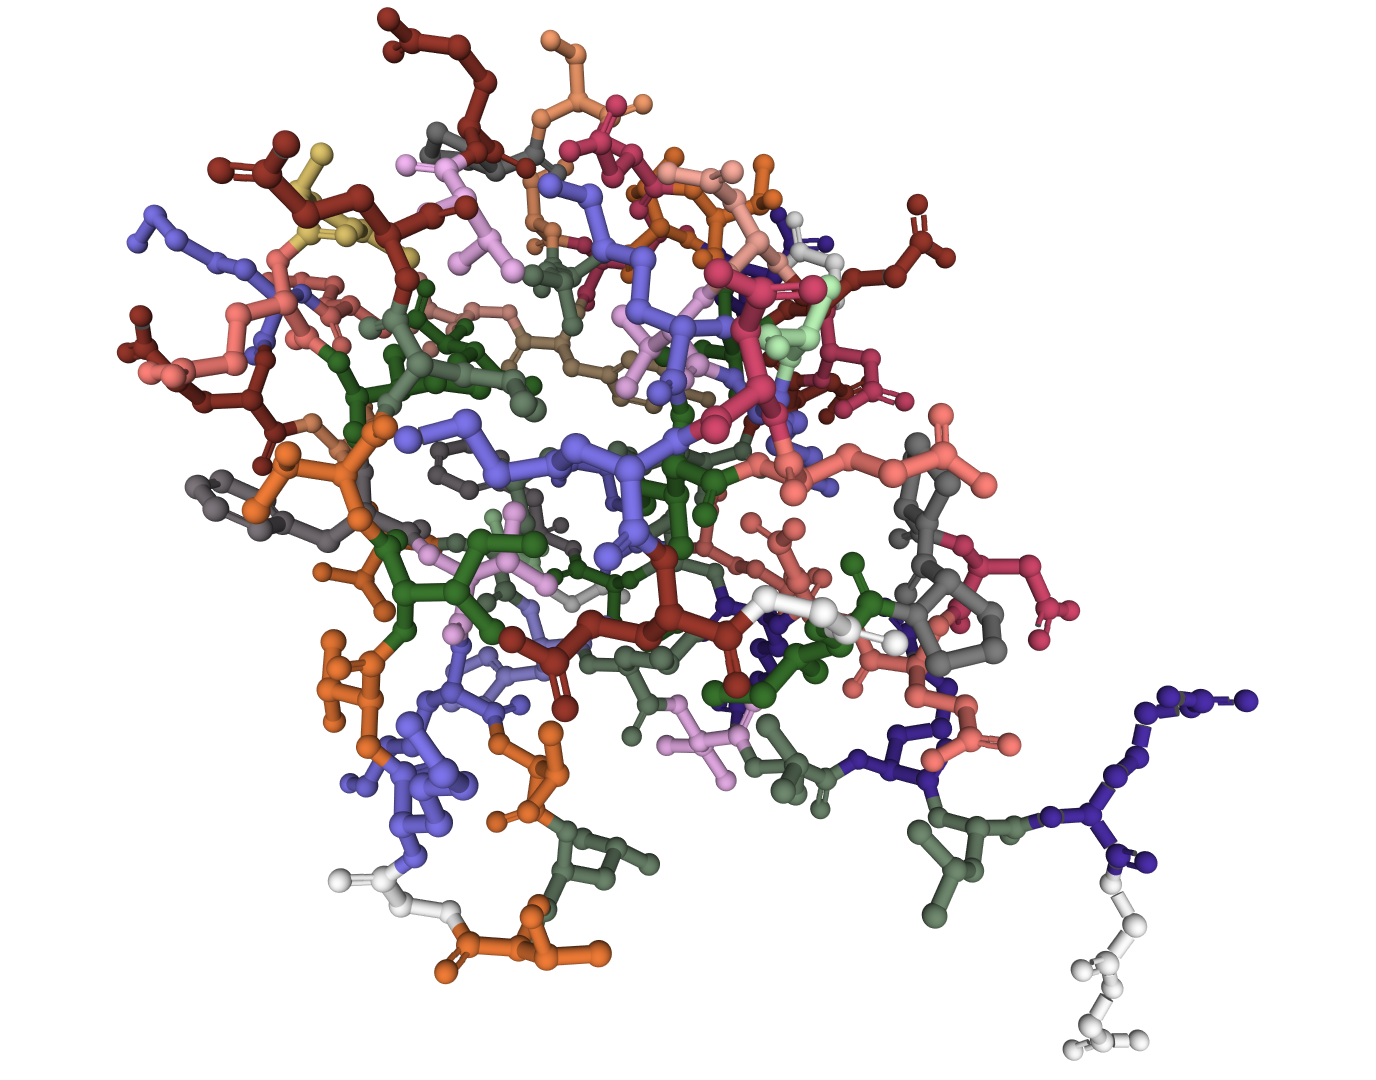
\includegraphics[width = 0.49 \textwidth]{graphics/ubq_balls.png}
  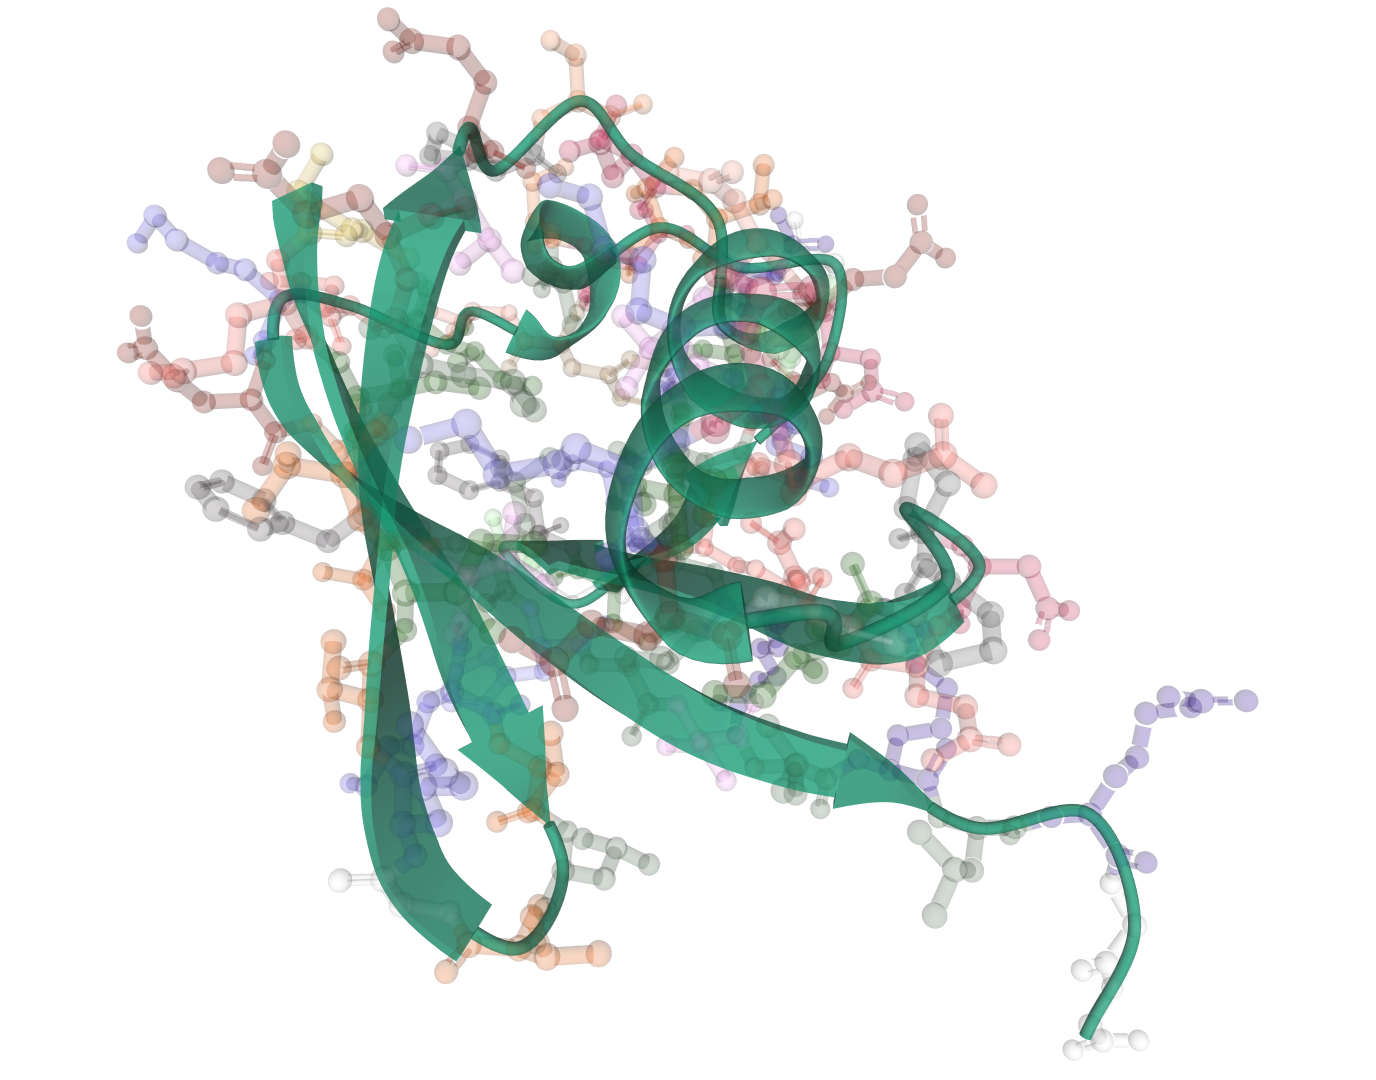
\includegraphics[width = 0.49 \textwidth]{graphics/ubq_ribbon.png}
  \caption{Conformation of ubiquitin. Each ball and stick respectively represent an atom and a covalent bond, colors correspond to residues (left). 
  Additional ribbon diagram highlighting the linear arrangement of residues is superimposed on the atoms (right). 
  Both images were created with Mol*~\cite{mol}.}
  \label{f:ubq}
\end{figure}


Molecular dynamics (MD) simulations offer a promising approach to deriving dynamics of a protein
from easily obtainable information, such as its amino acid sequence. 
In a traditional MD algorithm, which dates back to the 70s~\cite{md_nature}, positions and velocities
of all atoms forming the protein are maintained explicitly. In subsequent steps they are updated 
by numerically integrating equations of motion. Those equations often boil down to calculating the net
force acting on each atom and simply applying Newton's second law of motion~\cite{md_aa}. 
The core of any MD model is defining force fields that govern how the atoms interact with each other
and fine-tuning them so that the results match experimental data.

The most limiting factor of MD simulations is reaching time scales relevant to biological processes.
During each step we can advance time by only so much before introducing artifacts and instability.
This usually limits the time step to the order of $10^{-15}$ seconds, which is $10^9$ times smaller than 
even the shortest relevant simulation lengths~\cite{md_aa}. 
Because of this limitation a single MD experiment can take many days or even weeks to finish 
and any significant speed-up of the algorithm's implementation would increase its range of applications. 

An example method of increasing available simulation time scales is to use coarse-grained representation of a protein. 
This requires dividing atoms into groups, e.g. by amino acid residue they come from, and then treating each group as one object. 
This can decrease the amount of computation required to process one step, but the biggest profit is that  
because of losing some details about the movement of individual atoms, we can greatly increase the time step 
before running into issues with stability~\cite{md_aa}. However, this comes at a cost of reduced accuracy
and increased complexity of the model and its implementation.


As part of this thesis we have reimplemented a coarse-grained MD model developed in the Institute of Physics of the Polish Academy of Sciences. The model and its implementation have been developed for over 20 years, starting in 2000 with a first version created to simulate ordered proteins~\cite{cg_1}, i.e. proteins that have a known, stable conformation. Then, in 2008, it was used to study stretching of proteins~\cite{cg_2} and lately, in 2018, extended to also simulate disordered proteins~\cite{QA_model}, which may have no stable conformation. In 2020, a more accurate method for disordered proteins was developed~\cite{PID}. The program in its current state has many flaws, the most important being that it's overcomplicated, which makes it hard to understand and even harder to extend with new functionalities. Some of this complexity comes from the model itself, but arguably most of it comes from poor programming practices and an obsolete programming language (FORTRAN 77), which doesn't provide enough high-level abstractions needed for such complex application. The authors of the program realized that it would be beneficial to reimplement this model in a modern, high-level language and this thesis is a summary of our efforts to produce readable, efficient and functionally equivalent code.


The rest of this thesis is organized as follows: In chapter 2, we provide basic information about the model itself. In chapter 3, we discuss the original implementation, list some of its features and comment on its issues, this way we provide justification for the project and make it possible to later argue why the new implementation is qualitatively better. Chapter 4 is the focal point of this thesis, it presents the new design as well as comparison of how the features are implemented in both programs. It also describes how we achieve better parallelism and discusses some new interesting optimizations. Chapter 5 contains some benchmarks' results and their analysis --- these provide the most objective advantages of the new program over the old one. In chapter 6 we give an overview of individual contributions among the team and in chapter 7 we describe additional files attached to this thesis. 
\chapter{The model}\label{c:model}

In this chapter we discuss the basics of the molecular dynamics model that was implemented as part of this thesis. We start by describing how the proteins are represented and explaining what governs their movements. Next we describe 3 substantially different examples of potentials that can be applied in this model.

\section{The basics} 
The model is coarse-grained, which means that it groups entire amino acids into individual pseudoatoms. Since proteins are made of chains of amino acids, this model treats them as chains of pseudoatoms. The entire complexity of the model is in the definitions of its potentials, or equivalently, its forces. Each potential is simply a formula that takes all pseudoatoms' positions and outputs the force vector for every one of them. Once we have all the potentials, we can define how the positions evolve with time --- the movement of each pseudoatom is described by the Langevin equation of motion:

$$ m\frac{d^2 \vec{r}}{d^2t} = \vec{F} - \gamma \frac{d\vec{r}}{dt} + \vec{\Gamma}$$

It says that the mass times acceleration is equal to the sum of 3 vectors. The first one is the net force arising from all the potentials. The second one is a negative constant times velocity, which results in motion damping, where the faster a pseudoatom moves, the faster it decelerates. The third one is a random gaussian vector with variance proportional to external temperature, which simulates randomly bumping into jiggling water molecules. Simulation is essentially a process of numerically solving the equations of motion using selected numerical scheme. It simply boils down to summing all the forces acting on each pseudoatom, then adding motion damping and random noise and finally applying some numerical integration algorithm. 

\section{Examples of potentials}
Since the whole complexity of the model lies in its potentials, let's review a couple examples.

\begin{itemize}
    \item \emph{Bond angle} potential for disordered parts.
    This is an example of a local potential, which means that interactions happen only between pseudoatoms that are close to each other within one chain. In this case, we can limit ourselves to considering all triples $(i-1,i,i+1)$ of consecutive pseudoatoms. Local potentials are introduced to maintain the stiffness of the chain. 
    The value of the force arising from this particular potential depends on the planar angle formed by pseudoatoms $(i-1,i,i+1)$. It is a value of a sixth degree polynomial evaluated at that angle and the coefficients of this polynomial depend on what amino acids make up this angle. This gives 9 different polynomials in total.
    
    \item \emph{Quasi-adiabatic} potential. This potential is not local, which means that it can create interactions between any pair of pseudoatoms that will be close enough to each other. It is based on the idea of a contact, where contacts are determined dynamically on the basis of several criteria. The first criterion is the distance between a given pair of amino acid residues. The second criterion is geometric and it is required to check the corresponding angles between specific chemical bonds present in amino acids. Since we do not remember the positions of all atoms in the model, but only the positions of entire amino acid residues, the angles are reconstructed on the basis of the positions of adjacent residues in the chains. The third criterion is the limit on the number of contacts a given amino acid can create. Amino acids are divided into several groups depending on their chemical properties, and the limits for these groups differ. The contacts are created quasi-adiabatically, that is, once formed, the force does not immediately increase to its maximum value, but increases gradually. The same method is used for breaking contacts. This is done to avoid numerical instabilities, but it means that this potential has an internal state which the simulation needs to remember.

    When a contact is established, the force between two pseudoatoms in contact depends only on the distance between them, which makes computing this potential quite fast. 
    
    \label{ref:disul} There is also a special type of contact that can form --- a disulfide bridge. It can only be formed by a pair of cysteines, which are one of the amino acids. These have an additional criterion for creation. A cysteine cannot be a part of more than one disulfide bridge.
    
    \item \emph{Pseudo-improper dihedral (PID)} potential. The PID potential was introduced as a substitute for quasi-adiabatic. In fact it achieves higher accuracy when compared with experimental results. PID makes contacts only depending on the distance between the pseudoatoms, but the value of the acting force depends on complicated geometric criteria that take into account the positions of the pseudoatoms that are to interact with each other and their neighbors in the chains. Contacts are no longer created quasi-adiabatically, which makes this potential stateless, but in each step of the simulation more calculations need to be made to compute the acting force, making the overall simulation slower in practice.

\end{itemize}




%%% REFERENCE IMPLEMENTATION
\chapter{Reference implementation}\label{c:ref_impl}

\section{Overview}

The reference implementation has been written in FORTRAN 77. It consists of a single file with ~8000 lines of code. Because of old technology, long program  development history and disregard for good programming practices, its code is difficult to understand. However, we haven't found any significant bugs in the code.


\section{Features}
We provide a list of the most important features of the program.

\subsection {Potentials}

Program implements all potentials defined in the model. However, their code is poorly separated. Different physical potentials are often implemented in the same subroutine for convenience and there is a lot of communication through global variables. All of this makes it hard to understand the non-trivial interactions between potentials. 

Since calculating forces is the heaviest part of all computations, most of the potentials are parallelized using OpenMP (see section \ref{new:parallel}), however virtually all potentials suffer from a simple race condition and a few of the more complicated ones are affected by a more subtle race condition that is much harder to eliminate. Even if those were fixed, the multi-threaded version is by design non-deterministic, which makes it much less suitable for research. 

\subsection {Verlet list} \label{ref:verlet}
Many potentials depend highly on the distance between two residues. When they are far away from each other, their mutual interaction is too weak to be relevant for simulation. Therefore, in order to reduce computation time, program maintains a list of pairs of residues that are close enough to possibly have impactful interaction. This solution is called Verlet list and it is one of the key features of this implementation. 

Unfortunately, different potentials require different pairs to be included in the Verlet list (not only based on distance) and they sometimes need to assign additional data to the entries in the list. The program has 4 different lists, 2 of them store additional data and one needs this data to be persistent after update while the semantics of this data depend on the simulation scenario. All of this makes the code responsible for building the lists very hard to understand (see the last example in subsection \ref{ref:flaws}). 

\subsection {Simulation protocols}
Program offers several simulation protocols corresponding to different real life situations:
\begin{itemize}
    \item Default --- proteins are located in infinite space and no external forces act upon them.
    \item Folding --- an ordered protein is simulated in infinite space and the simulation ends when all native contacts become active (meaning that all pairs specified as native contacts are closer to each other than a given threshold).
    \item Stretching by Atomic Force Microscope tips --- the first and the last residues are pulled apart along the line connecting them.
    \item Walls --- simulation space is limited by walls. Implementation offers a choice between a box (limits to all dimensions) and pair of walls perpendicular to Z axis. The walls limiting Z dimension may be customized. There are three kinds of box walls in program, each interacting differently with residues, as described in the next subsection.
    
\end{itemize}

\subsection {Boundary conditions}\label{ref:boundary}
When running simulation with walls, one can choose between three kinds of walls perpendicular to Z dimension. Other walls, when they exist, are always repulsive:
\begin{itemize}
    \item Face-centered-cubic walls --- each wall is made of two layers of immovable beads in a face-centered-cubic lattice. They interact with residues via Lennard-Jones potential.
    \item Flat attractive walls - when residue gets close to wall, it gets attracted by artificial bead on the other side of wall with the same X and Y coordinates.
    \item Sticky harmonic walls - residues closer to wall than given cutoff are harmonically attached to it.
\end{itemize}

The user can also enable periodic boundary conditions (PBC) individually for each dimension. If PBC is enabled for a dimension, then the space is wrapped around this dimension with the period equal to the size of the simulation box, so the distance between two walls of the simulation box that are perpendicular to this dimension is zero.   


\subsection{Checkpoints}
Program allows saving checkpoints at intervals of given length. Checkpoints may be used for resuming the simulation. However, not all data is saved, for example pseudoatoms' acceleration vectors and adiabatic counters used by the quasi-adiabatic potential are lost with each restart, which makes this feature incomplete. This issue has led to incorrect results and instability in the past. 

\section{User interface}

The program can be interacted with only via files in its working directory. It doesn't use standard input and uses standard output only to print errors.

\subsection{Input}\label{ref:input}

The only argument of the program is the name of the main input file. This file contains key-value pairs of different parameters and/or the names of other input files that need to be read. There are over 100 parameters, most of them can be divided into 3 categories based on their type:

\begin{itemize}
    \item Boolean --- these mostly govern \emph{what} the program needs to do, i.e. which potentials should be present, which simulation scenario should be chosen, what kind of output should be generated. They can also enable numerous minor tweaks in the model. Unfortunately some combinations of choices for these values are invalid (either because it doesn't make physical sense or because the implementation doesn't support it), but the program doesn't validate its input.
    \item Integer --- they determine the number of simulation steps that should pass between different events, for example how often to save a checkpoint or how many steps to wait before triggering wall oscillations.
    \item Floating point --- these are mostly physical constants used in the calculations of forces in the model.  
\end{itemize}

All those parameters have default values defined at the beginning of the program. 


The remaining input data is provided by specifying the names of other input files: \texttt{pdbfile}, \texttt{seqfile}, \texttt{paramfile}, their contents are described below:

\begin{itemize}
\item \texttt{pdbfile} is the native conformation in the PDB~\cite{pdb} format.

\item \texttt{seqfile} provides information about a disordered protein. It contains information about the number of chains and their amino acid sequences in one-letter format. Additionally, each chain has a list of names of its contact map files. A contact map is yet another file which holds information about an ordered region within a chain. 

\item \texttt{paramfile} stores remaining model parameters. It's mostly used to pass arrays into the model, for example the coordination numbers for each amino acid or 63 coefficients for the bond angle potential.
\end{itemize}

All of the above files can be read correctly only if they conform to a very strict format, which doesn't allow for additional whitespace characters or comments.

\subsection{Output}
Program may produce several output files:

\begin{itemize}
\item \texttt{outfile} is the main simulation output. It comprises various statistics, for example total system energy or parameters regarding the protein's shape.

\item \texttt{savfile} contains output structure in PDB~\cite{pdb} format.

\item \texttt{mapfile} is a contact map for the resulting structure (see \texttt{seqfile} in subsection \ref{ref:input}).

\item \texttt{rstfile} is a checkpoint needed for restarting the simulation.

\end{itemize}

\section{Code quality}

Reference implementation code has many flaws due to limitations of the used language and poor programming practices.

\subsection{FORTRAN 77 limitations}
Language limitations include:
\begin{itemize}
    \item Lack of object oriented programming support.
    \item Lack of basic data structures (such as set or map).
    \item Variable naming limitations.
    \item No functionalities for easy input parsing.
    \item In the standard format, lines are limited to 72 characters.
\end{itemize}

\subsection{Code flaws} \label{ref:flaws}
Poor programming practices include:
\begin{itemize}
    \item Possible race conditions.
    \item Excessive usage of global variables (around 250 in total).
    \item Insufficient code partitioning, e.g. the main simulation loop spans more than 600 lines. 
    \item Subroutines having multiple independent concerns, e.g. VAFM procedure handles one of the Atomic Force scenarios as well as one kind of wall interactions.
    \item Small amount of comments
    \item Inconsistent indentation, often caused by the 72 character limit.
    
    \item Obscure names of variables without comments, for example:
    \begin{lstlisting}[firstnumber=32, title=Names of some global variables in code]
common/verl/oxv(3,len),vrcut2sq,af,kfcc(3,len*500,2),kfccw,menw
common/cmap/kront,krist(3,len*500),klont,klist(3,len*50),lcintr
common/cmp2/kcont,kcist(3,len*500),kqont,kqist(4,len*1500,2),jq
    \end{lstlisting}
    
    \begin{minipage}{\textwidth}
    \item Assigning different meanings to one variable, for example:
    
    \begin{lstlisting}[firstnumber=3977, title=\texttt{z0temp} used as an array of z-axis positions]
do ib=1,men
    z0temp(ib)=z0(ib)
    ksorted(ib)=ib
enddo
call sort2(men,z0temp,ksorted) ! sort by z0
    \end{lstlisting}
    
    \begin{lstlisting}[firstnumber=6835, title=\texttt{z0temp} used as an array of adiabatic counters]
if(r.gt.sigma1(9)*1.5) then
    if(z0temp(i).gt.0) then
        z0temp(i)=z0temp(i)-1
    else
        z0temp(i)=0
        ipw(1,ip)=0
    endif
else
    if(z0temp(i).lt.ad) then
        z0temp(i)=z0temp(i)+1
    endif
endif
    \end{lstlisting}
    \end{minipage}
    
    \item Multiple violations of Don't Repeat Yourself (DRY) rule, for example:
    \begin{lstlisting}[title=This snippet appears 14 times]    
if(lpbcx) dx = dx-xsep*nint(dx*xinv)
if(lpbcy) dy = dy-ysep*nint(dy*yinv)
if(lpbcz) dz = dz-zsep*nint(dz*zinv)
    \end{lstlisting}
    
    
    \begin{minipage}{\linewidth}
    \item Complicated control flow using \texttt{goto}, for example:
    \begin{lstlisting}[title=Control flow structure of the main part of \texttt{update\_verlet\_list} subroutine]
9797    continue
        if(...) then ! find native contacts
            if(...) then
                goto 9797
            else if(...) then
                goto 1129
            endif
        endif
        ! 3579 is the label for "the rest" of contacts
        if(...) goto 3579
        if(...) then ! 3580 skips electrostatics
            if(...) goto 3580
            if(...) goto 3579
        endif
        if(...) goto 3579
        if(...) goto 9696 !no need 2 keep kqist for pid
9898    continue
        if(...) then ! find non-native c.
            if(...) then
                goto 9898
            else if(...) then
                !if(lpid) goto 3579
                goto 1129
            endif
        endif
9696    continue
        ! make a new non-native contact
        if(...) then
            if(...) goto 3580
        else
            goto 1129 ! TODO check if it works for lpid
        endif
            ! electrostatic, disulfide or repulsive contacts
3579    continue
        if(...) goto 3581 !skip ssbond and electr
        if(...) then
            goto 1129
        endif
3580    continue
        if(...) then
            goto 1129
        endif
3581    continue
        if(...) then ! REPULSIVE CONTACT
        endif
1129               
    \end{lstlisting}
    \end{minipage}
\end{itemize}



%%% NEW IMPLEMENTATION
\chapter{New implementation}\label{c:new_impl}

In this chapter we present the main contribution of this thesis: the new and improved implementation of the model. First, we provide an overview of the program and the design philosophy behind it. Then, we go over the features of the reference implementation and discuss how they are implemented in the new program. Finally, we present performance optimizations that we have developed in addition to the already present ones.

\section{Design}\label{new:design}

Reference implementation provides the means of simulating a number of altogether separate scenarios, which are nevertheless joined together in the form of a single program. These share a common foundation in the form of file parsers, forces and other ancillary features. It is natural to extract this foundation into a library of components which the users can freely use to construct their own scenarios. Our efforts focused on developing a system of abstractions, which would govern the structure of this library and would allow users to develop their particular simulation scenarios without having to know the ins and outs of the implementation, as well as let them easily create new components. We have arrived at a following set of design choices:

\begin{enumerate}
    \item There should be a ``centerpiece'' class which represents the entire simulation. We also considered the alternative of providing all the components separately and letting users link them, as though they were essentially functions, however we felt that this kind of code would become burdensome to write and not provide any benefits to the end user.
    \item One should be able to instantiate it with ease, using objects representing the initial state and the parameters of the simulation generated by an array of provided file parsers.
    \item The simulation object should provide a way to add various objects representing forces that act on the pseudoatoms, as well as any other computations that should happen during a simulation step. These objects should be independent of each other as much as possible.
    \item Performing a simulation step should be straightforward, preferably a single function call, as opposed to a number of function calls spread out in the code in multiple places.
    \item Implementation details should be hidden from the user.
\end{enumerate}

With these changes, the intricate user interface of the original program has been replaced with a more declarative one which should better convey the structure of the simulation scenario in question. Listing \ref{list:new_prog} shows an example of a simulation scenario composed of different library components:

\begin{lstlisting}[language=C++,caption=Example scenario that simulates an ordered protein]
int main() {
    ifstream param_file("data/parametersMJ96.txt");
    auto params = param::LegacyParser().read(param_file);
    
    ifstream pdb_file("data/1ubq.pdb");
    auto atomic = pdb::Parser().read(pdb_file).asModel();
    atomic.addContactsFromAtomOverlap();
    auto model = atomic.coarsen();

    Random rand(448);
    // Initial conditions
    model.morphIntoSAW(rand, false, 0.0, 4.56*angstrom, true);
    model.initVelocity(rand, 0.35 * eps_kB, false);

    Simulation simul(model, params);

    simul.add<Random>(rand);
    
    // Add the integrator 
    simul.add<LangPredictorCorrector>(0.005 * tau);

    // Add forces
    simul.add<Tether>(true);
    simul.add<NativeBA>();
    simul.add<ComplexNativeDihedral>();
    simul.add<NativeContacts>();
    simul.add<PauliExclusion>();

    // Add hooks
    auto total = 15000.0*tau;
    simul.add<ProgressBar>(total, 10.0*tau);
    simul.add<ExportPDB>("result.pdb", 100.0*tau);

    // Run the simulation
    simul.step(total);
    return 0;
}
\end{lstlisting}\label{list:new_prog}


It should be quite clear how an end user of the library can load the requisite resources, operate on them, instantiate a simulation object with them, choose an integrator, add force fields and additional actions to perform and finally run the simulation. In contrast, constructing similar scenario in the original program would require setting appropriate global variables and by extension understanding the semantics and interactions of all provided settings of the program. Adding a new scenario would require adding these options manually to the list of global variables, as well as having to modify potentially unrelated code in order to accommodate the addition, potentially breaking it.

We will now elaborate on the implementation details of this system.

\subsection{\texttt{Simulation} class}
\texttt{Simulation} class is the centerpiece of the library: it provides a declarative interface for preparing and running the simulation and hides the implementation details from users. For an end user, two methods are available.

The method \texttt{step(double t)} performs a number of simulation steps, i.e. computes forces (see subsection \ref{new:impl_model} for details), runs hooks, integrates the equations of motion and advances the internal clock by $\Delta t$ until the total of $t$ time has passed.

The method \texttt{add<T>(x1, ..., xn)} is more involved. It adds an object \texttt{T(x1, ..., xn)} to the simulation. We wanted to achieve a uniform interface, so this method does different things depending on the type \texttt{T}. If it is a force, we add it to the list of forces. If it is an integrator, we replace the current integrator with it. This is internally achieved by using a heterogeneous collection. The implementation also automatically manages memory. Although in the original implementation the memory management was not an issue, this was rather due to it being statically allocated, which created a host of other problems, such as possible overflows or excessive memory usage of the program.

Objects added to the simulation may require access to other objects present in the same simulation. For example, non-local forces naturally require access to the Verlet list and all forces need access to \texttt{State}, which holds pseudoatoms' positions. This is handled by two mechanisms:

\begin{enumerate}
    \item Objects may inherit an interface \texttt{SimulVar} with a method \texttt{bind(Simulation\&)}, which completes the initialization of an object when it is added to a simulation.
    \item Method \texttt{simul.var<T>()} allows any object to obtain a reference to the object of type \texttt{T} added to the simulation. If such an object does not exist yet, it will be constructed and added. Thanks to this setup, the user of the library does not have to manually add objects that are used internally by forces and hooks. For example, it is not necessary to explicitly add the Verlet list, the first non-local force will add it automatically.
\end{enumerate}

We also prevent adding or accessing simulation variables after the simulation has started. This has the effect of requiring component developers to fetch all the necessary dependencies during the binding phase. So understanding all the inter-component dependencies requires only reading the implementations of the \texttt{bind} methods.

The final interface is type- and memory-safe, concise, hides implementation details and yet is extensible.

\subsection{I/O and model preparation}
Before the simulation can be started, one needs to prepare the state, which includes initial positions and velocities of the amino acids. It is also necessary to prepare model parameters, such as amino acid radii or various force coefficients. In the Fortran implementation, the preparation layer and the simulation layer of the program were tightly connected, in particular they operated on the same global variables and used the same data formats. We argue that they should rather be separated as much as possible. For one, their design philosophies are different: preparation layer, by virtue of being visible to the user, must be convenient to work with, whereas the simulation layer objects are hidden behind \texttt{Simulation} and are subordinated to performance considerations. Moreover, file parsers and other intermediate objects should not depend on the parts of the program which use them. In the new design, we have achieved such a separation --- the only part where the layers interact with each other are \texttt{Model} and \texttt{Parameter} classes, which represent state and the parameters of the simulation respectively, and which form an input to the \texttt{Simulation} object. We provide parsers for all files used in the original program, as well as a custom, modular parser of PDB files. It allows generating better stardards-complying and comprehensive output PDB files compared to the original implementation, which produced files that caused issues with third-party software that analyzed them. Parsers and data objects generated by them have been separated, so that new file formats can be introduced by simply writing a parser class, without having to change any other parts of the code.

\subsection{Simulation hooks}
We also provide a uniform interface for various actions that are performed after the evaluation of all force fields --- the class \texttt{Hook} with a method \texttt{void execute()}. Users can define custom classes deriving from \texttt{Hook} and add it to the \texttt{Simulation} object via \texttt{add} method, which will invoke them automatically after the integration of the equations of motion.

\section{Abstractions in the performance-critical code}\label{new:abs}
Many of the design decisions taken during the development of the reference program that resulted in inelegant code were dictated by performance considerations. Given that much of the time developing an extension to the library, in particular introducing new force fields, is spent writing performance-critical code, it was crucial to show that legibility of the code, use of abstractions and comfort of the programmer needs not be sacrificed for the speed of the simulation.

\subsection{Linear algebra}
In order to make the linear algebra code more concise and natural we used the \emph{Eigen} library \cite{eigen}. It exposes a user-friendly interface for performing calculations, utilizing the flexibility of C++ operator overloading and expression templates, which make the resulting code expand to a Fortran-equivalent during compilation. Example is provided in Figure \ref{f:dihedral}

\begin{figure}[ht]
    \noindent
    \begin{minipage}{.5\textwidth}
      \begin{lstlisting}[language={[77]Fortran}]
      ux1=rx(2)-rx(1)
      uy1=ry(2)-ry(1)
      uz1=rz(2)-rz(1)
    
      ux2=rx(3)-rx(2)
      uy2=ry(3)-ry(2)
      uz2=rz(3)-rz(2)
    
      ux3=rx(4)-rx(3)
      uy3=ry(4)-ry(3)
      uz3=rz(4)-rz(3)
    
      vx1=uy1*uz2-uz1*uy2
      vy1=uz1*ux2-ux1*uz2
      vz1=ux1*uy2-uy1*ux2
      vv1=vx1*vx1+vy1*vy1+vz1*vz1
    
      vx2=uy2*uz3-uz2*uy3
      vy2=uz2*ux3-ux2*uz3
      vz2=ux2*uy3-uy2*ux3
      vv2=vx2*vx2+vy2*vy2+vz2*vz2
    
      v12=vx1*vx2+vy1*vy2+vz1*vz2
      v12=v12/sqrt(vv1*vv2)
      v12=min(v12,1.d0)
      v12=max(v12,-1.d0)
      phi=dacos(v12)
    
      di=vx1*ux3+vy1*uy3+vz1*uz3
      if(di.lt.0.d0) phi=-phi
      \end{lstlisting}
    \end{minipage}%
    \begin{minipage}{.5\textwidth}
      \begin{lstlisting}[language=C++]
      Vector u1 = r2 - r1;
      Vector u2 = r3 - r2;
      Vector u3 = r4 - r3;
      
      Vector v1 = u1.cross(u2);
      Vector v2 = u2.cross(u3);
      
      double cos_phi = v1.dot(v2) / sqrt(v1.squaredNorm() * v2.squaredNorm());
      
      cos_phi = max(min(cos_phi, 1.0), -1.0);
      double phi = acos(cos_phi);
      if (v1.dot(u3) < 0.0) phi = -phi;
      \end{lstlisting}
    \end{minipage}
    \caption{Comparison of Fortran (left) and C++ (right) implementations for the computation of dihedral angle between four consecutive pseudoatoms. The C++ version is much shorter and better conveys the intent behind the function.}
    \label{f:dihedral}
\end{figure}


\subsection{Force kernels}
Many of the force fields present in the model use the Lennard-Jones potential \cite{lj} with varying potential depths and values of the minimum radius. In the Fortran code, these parameters are global, and the code computing the forces acting on each residue and the potential energy is replicated every time, sometimes in a slightly modified form. We recognized this as an opportunity to extract it and similar constructs into \emph{force kernels}, which hold the parameters necessary for computing forces and potential energy. By implementing the computations of the potential energy and forces as inlined functions as opposed to placing them in \texttt{*.cpp} file, the function call overhead is not incurred. Because the parameters for the evaluation are now in one place, one needs to know less of other parts of the code. Finally, it allows us to implement more complex force fields in a more elegant fashion, by storing many such kernels in the force field class and invoking the force/energy computation forces as required.

\subsection{Physical units}
Physics simulations require storing various physical quantities, such as forces, energies and distances. They are usually represented in internal units as opposed to SI. In the Fortran version, this aspect of the implementation was handled in an inadequate fashion. Most inputs were assumed to be in the internal units, except for the distance values read from PDB files and certain config parameters, which were scaled. This kind of approach is inflexible, as in order to change the internal units one would have to change many of the input files and simulation parameters. It is also difficult to convert standard units to the internal units and back, because some of internal units are not explicitly assigned values in terms of SI units. One can easily introduce errors by forgetting what the proper units of a particular quantity are. In fact, we have found one such bug in the original code.

We resolved all these issues by having a single file \texttt{Units.hpp} with all the units, and specifying all the physical quantities present in the code with the appropriate unit. Now, changing the units of the simulation requires changing values in a single file, and it is harder to introduce bugs. We also define all SI units, which makes the conversion between internal and standard units easy.

\section{Features}\label{new:features}

In this section we go through some of the features of the reference program and briefly discuss how they are implemented in the new program.

\subsection{Verlet list}

In contrast with the reference program, Verlet list is completely free of potentials' implementation details. It has a simple interface. Objects of class \texttt{NonlocalForce} specify what is their required cutoff distance and provide their implementation of \texttt{vlUpdateHook}, which is a function that will be called each time the list is updated. The list holds only pairs of indices pointing to two pseudoatoms that may be closer than the cutoff. If some potential needs to keep some data for each pair in the list, it needs to maintain it itself, usually by updating its internal list in the \texttt{vlUpdateHook}. This greatly simplifies Verlet list's implementation and the clear interface increases readability. Additionally, we have implemented significant optimizations for updating the list, which we describe in subsection \ref{opt:verlet}.

\subsection{Simulation protocols}

Each simulation protocol translates to a subset of objects added to the \texttt{Simulation} object. If one needs wall interactions, one should add the relevant potential to the simulation. If one wants the simulation to end once all native contacts are present, it can be achieved by using a simple \texttt{Hook}, which holds a reference to \texttt{NativeContacts} object and after each step it checks the number of present native contacts. This design makes it easy to see what particular simulation is supposed to do by just looking at the code that builds the \texttt{Simulation} object.

\subsection{Boundary conditions}

Wall interactions are implemented using \texttt{Force} interface, just like all other potentials. A small \texttt{Topology} class deals with concerns surrounding the simulation box. It provides current positions of the box's walls and can calculate the shortest vector between two points in space, which matters only if the periodic boundary conditions are enabled.

\subsection{Checkpoints}

Saving and loading a checkpoint requires being able to save and load the internal state of all objects added to the simulation. The internal state can be defined as the data that can change in one step and then be used in another step. Most notable examples include pseudoatoms' positions and their derivatives, adiabatic counters used in quasi-adiabatic potential and dimensions of the simulation box. Verlet list also satisfies this definition, because we reuse it between steps for performance reasons, but it is not necessary to save it, since it can always be rebuilt from other data. 

We extended \texttt{SimulVar} interface with two methods: \texttt{serialize} and \texttt{deserialize}, which respectively save and load internal state using a human-readable format. This allows us to easily serialize and deserialize the whole simulation object using polymorphism.

\section{Parallel processing}\label{new:parallel}

Both reference and new implementation use the OpenMP~\cite{openmp} library. It provides compiler directives and environmental variables that form a high-level API for portable shared memory parallelism. Its biggest advantage is its simplicity. If the user wants to run a loop in parallel, all it takes is to write one short directive above and the compiler will automatically insert code that prepares a thread pool, distributes loop iterations between threads and joins them after. 

The reference implementation used OpenMP to parallelize loops that are responsible for most of the computations i.e. calculating forces and integrating the equations of motion. Each loop is parallelized individually, which generates many unnecessary synchronization barriers, slowing down the simulation.
Another issue is that the authors did not protect shared data, which resulted in multiple race conditions. One could avoid those by using atomic instructions and proper synchronization techniques, but even then the original design would suffer from non-determinism, because there are some potentials where creation of one contact prohibits the creation of another. 

We decided to also use OpenMP for the new implementation, because it is portable, simple and familiar to the future users. However, instead of  handling each force individually, we used it to implement a simple abstract model of computation that is restrictive enough to be easily parallelizable, thread-safe and deterministic, while powerful enough to enable implementing all forces in a way that efficiently makes use of multiple threads. 

\subsection{Model of computation}

All forces must implement the \texttt{Force} interface. It requires implementing two methods: \texttt{asyncPart} and \texttt{syncPart}, both return \texttt{void} and take one argument --- a reference to an object of class \texttt{Dynamics}. It holds intermediate results of force computations, namely the total potential energy and the total force vector for each pseudoatom. All it takes to compute a single force is to first call its \texttt{asyncPart} and then its \texttt{syncPart}. The result will be added to the provided \texttt{Dynamics} object. These two methods have different semantics and their implementations must adhere to different rules:

\begin{itemize}
    \item \texttt{asyncPart}: This method is called in a multi-threaded setting. Data that is accessed in \texttt{asyncPart} by more than one \texttt{Force} class must not be modified, except for the \texttt{Dynamics} object provided in the argument. The entire body of this function should consist of one or more \texttt{for} loops, each prepended with \texttt{omp-for} directive.
    
    \item \texttt{syncPart}: This method is called in a single-threaded setting and it is guaranteed that it will be called after all other \texttt{asyncPart} computations finished. When there are many forces in the simulation, their \texttt{syncPart}s will be called in the order in which they were added to the simulation, so this order is fully controlled by the user. There are no limitations on the implementation, but obviously for efficiency it must be kept as fast as possible. 
\end{itemize}


The general idea is simple. As much of the computations as possible should be in \texttt{asyncPart}, but this method is much more constrained. Still, most of the potentials can be implemented without using \texttt{syncPart} at all. Most notably, all the potentials that are \emph{functional} in nature, meaning that they do not have any internal state and do not modify any data outside of the \texttt{Dynamics} object. 

\subsection{Implementing the model}\label{new:impl_model}

Calculating the forces using the interface above is straightforward when using OpenMP. The only interesting thing is ensuring that the code in \texttt{asyncPart} can freely modify the \texttt{Dynamics} object passed as an argument. The idea is to create a separate \texttt{Dynamics} object for each thread and combine them at the end in a critical section. Creating a private copy of an object for each thread can be done easily by using \texttt{threadprivate} directive, which will handle it in a way that is invisible to the user. Usually it works by putting it in Thread Local Storage, but this is dependent on architecture and library implementation. 

The whole code that implements this model of computation is shown in Listing \ref{list:parallel}.

\begin{lstlisting}[caption=Implementation of the described computation model]
#pragma omp parallel {
    dynamics_tp.clear();
        
    for (Force* force: forces) {
        force->asyncPart(dynamics_tp);
    }
    
    #pragma omp critical {
        state.updateDynamics(dynamics_tp);
    }
}

for (Force* force: forces) {
    force->syncPart(state.dynamics);
}
\end{lstlisting}\label{list:parallel}

\subsection{Example}\label{new:example}
Here we will review a more complicated example of two forces using the model of computations described above. The \texttt{NativeContacts} potential has a fixed list of pairs that interact with each other. Every such pair has a threshold distance and whenever the pseudoatoms are closer than this threshold, we say that there is a contact between them. Another potential --- \texttt{QuasiAdiabatic} --- dynamically creates and destroys contacts between pairs of pseudoatoms and calculates forces only between pairs in contact. One of the conditions for creating a contact is that each pseudoatom has a limit on the number of contacts it can be a part of. However, this limit also includes contacts defined by \texttt{NativeContacts}. 

All of this makes it challenging to parallelize those two forces. But the experiments show that an overwhelming part of computations in \texttt{QuasiAdiabatic} is spent on checking other conditions for contact creation and computing forces. An efficient solution is to do those computations in the \texttt{asyncPart}. There we create a list of potential contacts, which satisfy all conditions except for the limit on the number of other contacts. Finally, we check the last condition in \texttt{syncPart}, where we control the order of execution, which gives us determinism. All the computations relating to \texttt{NativeContacts} are performed in its \texttt{asyncPart}. There we calculate the numbers of native contacts for each pseudoatom and those values will be ready to use once \texttt{QuasiAdiabatic}'s \texttt{syncPart} is called. 
To sum up, we did not need to use complicated synchronization techniques and achieved determinism at a cost of doing a little part of computations sequentially.   

\subsection{More parallelism}\label{new:more_parallelism}
Parallelizing force computations is the most important factor when it comes to speed, since they take the most of the time. But there are other parts of code where the program spends a non-negligible amount of time and they can quickly become bottlenecks if they do not make use of multiple threads. Fortunately, almost all of them are simple loops over the pseudoatoms that need to be run after the positions are updated and before the next step begins, so they are trivially handled by using \texttt{omp-for} directive. The only exception is rebuilding the Verlet list, because it requires some non-trivial aggregation of results from different threads. Yet, it is still easy to implement by using threadprivate lists and combining them in a critical section.

However, there is one significant calculation which cannot be resolved that easily. In each step we need to generate a random gaussian vector for each pseudoatom, in order to simulate thermal noise from Langevin dynamics. If we want to keep determinism then we cannot simply parallelize it by distributing different pseudoatoms to different threads running at the same time. So it needs to be run by one thread, but in order to minimize the resulting bottleneck it could run at the same time as forces' \texttt{asyncPart}s. This can be easily achieved using \texttt{omp-task} directive, which creates a piece of code that will be executed by any thread that is free at the moment. That is why we extended the model of computation by adding \texttt{asyncTask} construct, which simply creates a task that will be executed by one thread in the parallel region that runs \texttt{asyncPart} computations.

In the current implementation the only use case of \texttt{asyncTask} is generating pseudorandom numbers, but one can easily imagine interesting optimizations that can be applied when the number of threads reaches the limit of available parallelism and adding more does not give any speedup. In such case, we can use \texttt{asyncTask} interface to perform additional computations basically for free. An interesting example is an \texttt{asyncTask}, which scans the Verlet list looking for pairs that will never get close enough before the next update, because they are already too far from each other, so they can be deleted.

\section{Optimizations}\label{new:opt}

In this section we describe some of the optimizations implemented in the new program.

\subsection{Verlet list}\label{opt:verlet}

The most important optimization in the reference program is the Verlet list (see subsection \ref{ref:verlet}). It was crucial that we implement it in the new program as well, but we also found opportunities for significant optimizations. Verlet list solves the following problem: given a cutoff $r$, in every step we would like to efficiently iterate through all the pairs of pseudoatoms $(i, j)$ which satisfy $dist(i, j) < r$. We define a Verlet list for a given cutoff $r$ and padding $s \geq 0$ to be a list of all pairs $(i, j)$ satisfying $dist(i, j) < r + s$. Building the list with a naive algorithm requires iterating through all pairs of pseudoatoms and computing their distances. For a large system this can take much longer than all other computations within one step. 

We can choose $s$ freely, but as it grows, so does the number of redundant pairs in the list, slowing down the process of iterating through pairs closer than $r$, which is the main part of all non-local forces' computations. However, when $s$ is big enough, it is possible to reuse the same list in some future steps, because in each step pseudoatoms move only a little. 

It is easy to quantify how big $s$ must be to safely reuse an old list. Let's define $d$ to be the biggest distance that any pseudoatom has moved since the list was constructed. By the triangle inequality we get that the biggest possible change of the distance between any two pseudoatoms is at most $2d$. It turns out that as long as $s > 2d$ we can still use the old list, because for any pair $(i, j)$ that now satisfies $dist(i, j) < r$, its old distance could not exceed $r + 2d$, so this pair is present in the old list, since $r + 2d < r + s$. 

By using this criterion it is possible to check if the old list can be reused. Since this requires much less computation than building a new list, choosing the padding provides a trade-off between the average time spent on calculating non-local forces and rebuilding the list. Predicting the optimal padding value is a very difficult task, because it is influenced by a myriad of factors, such as the number and the characteristics of non-local forces, shape of the simulation box, spatial distribution of pseudoatoms or even performance of the branch predictor. That is why both the reference and the new program rely on the user to empirically find the optimal padding.

The original program rebuilds the list using a naive algorithm that sequentially traverses all pairs of pseudoatoms. We implemented parallel versions of the naive algorithm and a more sophisticated cell-based algorithm. The latter starts building the list by partitioning the simulation box into cubic cells of side lengths equal to $r + s$. It is easy to show that if a pair of pseudoatoms should be in the list, then they are in the same cell or in the neighbouring cells. This way we can skip many pairs without calculating their distances, which can significantly speed up the list construction.

\subsection{Thermal noise}

As described in chapter \ref{c:model} and subsection \ref{new:more_parallelism}, each simulation step requires sampling a random gaussian vector for each pseudoatom. This is difficult to effectively parallelize if we want to maintain determinism, so we used the \texttt{asyncTask} construct to minimize the bottleneck by sampling the noise during force computations. It quickly turned out that further optimization was required, because enabling thermal noise greatly reduced the simulation speedup in multi-threaded setting, hinting that in each step generating the noise took more time than all the force computations. We introduced 3 improvements to mitigate this issue.

The first thing is to use a faster pseudorandom number generator (PRNG). We picked \texttt{xorshift64*} --- a fast, modern, general purpose PRNG of high statistical quality~\cite{xorshift}. Next we realized that it is easy to parallelize noise generation between 3 threads by sampling each coordinate separately. Finally, we noticed that the original implementation inefficiently uses the output from PRNG to sample gaussian vectors. Internally it relies on the Box-Muller transform~\cite{box-muller}, which operates in the following way.

Let $U_1, U_2$ be independent random variables with uniform distribution. Then, the variable $X = \sqrt{-2\ln{U_1}}\cos(2\pi U_2)$ is normally distributed.

This way we need two PRNG samples to generate one noise vector coordinate. After a quick Internet search, we found out that the Box-Muller transform actually states a stronger fact: if we also define variable $Y = \sqrt{-2\ln{U_1}}\sin(2\pi U_2)$, then $X$ and $Y$ are independent and normally distributed. Using this fact we implemented generating two vectors at once, which halved the number of required PRNG samples.

\section{Documentation}\label{new:docs}
Having in mind the difficulties in comprehending the original implementation, which limited its use and expansion, developing a comprehensive documentation of the program was a crucial part of the development process.

We have created an external documentation, which contains installation instructions, a tutorial, architecture of the library and the description of all the components. Documentation entries are automatically generated from Doxygen docstrings, and one can also add custom documentation pages, like the aforementioned installation instructions. Screenshot of the documentation is provided in Figure \ref{fig:docs}.

\begin{figure}
    \centering
    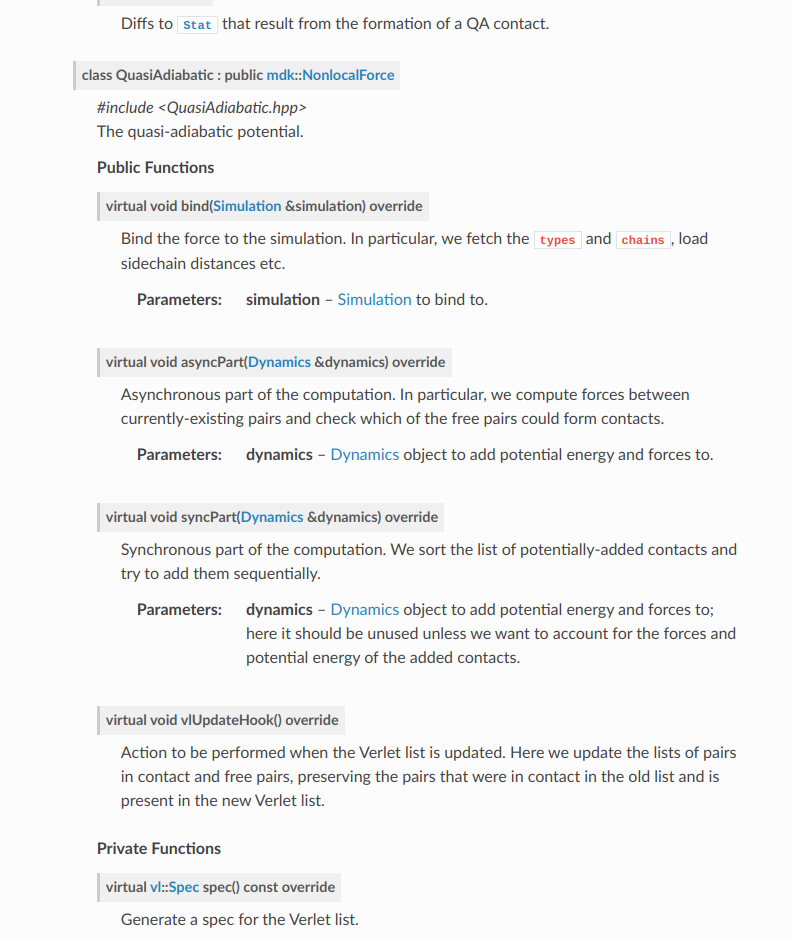
\includegraphics[width = \textwidth]{graphics/docs2.png}
    \caption{Screenshot of the documentation}
    \label{fig:docs}
\end{figure}

Moreover, in order to aid the modification of existing components, inline comments have been provided. However, we have observed that for the most part the documentation of variables in header files and the way the code is structured suffices to explain the semantics of the code, so this part of the documentation was for the most part limited to explaining certain sophisticated optimizations, like the algorithm for the cell-based construction of the Verlet list.

\chapter{Summary}\label{c:summary}

\section{Speed comparison}\label{summary:speed}

\definecolor{bblue}{HTML}{4F81BD}
\definecolor{rred}{HTML}{C0504D}
\definecolor{ggreen}{HTML}{9BBB59}

In this section we show the results of performance benchmarks.

\subsection{Single-threaded benchmarks}

First, we compared the performance of the reference program, the new program running in the legacy mode, which replicates the behavior of the reference version exactly, and the new program running in the release mode, which uses the new optimizations. We performed three benchmarks, for three values of the number of pseudoatoms. Figure \ref{f:bench_single} shows the normalized results of the benchmarks. As we can see, the performance of the new implementation is comparable with the performance of the Fortran version. In particular, the abstractions and the introduced quality-of-life improvements did not affect its speed considerably. At the same time, newly-introduced optimizations make it even faster.

\begin{figure}[ht]
\centering
\begin{tikzpicture}
\begin{axis}[
        width  = 0.95*\textwidth,
        height=8cm,
        ybar,
        bar width=20pt,
        ymajorgrids = true,
        symbolic x coords={small,medium,large},
        xtick = data,
        enlarge x limits=0.25,
        nodes near coords,
        ymin=0,
        ymax=1.7,
        legend style={
                at={(0,1)},
                anchor=north west
        },
        legend cell align=left,
        ylabel = {Steps/s (normalized)},
        xlabel = {Number of pseudoatoms}
    ]
\addplot [style={black,fill=rred,mark=none}]
	coordinates {(small,1.00) (medium,1.00) (large,1.00)};
\addplot [style={black,fill=bblue,mark=none}]
	coordinates {(small,0.98) (medium,0.90) (large,0.96)};
\addplot [style={black,fill=ggreen,mark=none}]
	coordinates {(small,1.12) (medium,1.16) (large,1.14)};
\legend{reference, legacy, release}
\end{axis}
\end{tikzpicture}
\caption{Single-threaded benchmarks}
\label{f:bench_single}
\end{figure}

\subsection{Multi-threaded benchmark}

Next, we compared the performance of the three aforementioned versions in a multi-threaded context. Figure \ref{f:bench_multi} shows the normalized results of the ``large'' benchmark. As we can see, the reference implementation benefited from the use of additional cores only by around 55\%, having stalled out at around 4 threads. Our implementation exhibits more favorable behavior, reaching a speedup 160\% higher than the Fortran version when using 8 threads. Combined with the fact that our implementation is slightly faster in the single-threaded setting, this shows that the new program is 193\% faster on this benchmark.

\begin{figure}[ht]
\centering
\begin{tikzpicture}
\begin{axis}[
        width  = 0.95*\textwidth,
        height=8cm,
        ybar,
        bar width=20pt,
        ymajorgrids = true,
        symbolic x coords={1,2,4,8},
        xtick = data,
        enlarge x limits=0.25,
        nodes near coords,
        ymin=0,
        legend style={
                at={(0,1)},
                anchor=north west
        },
        legend cell align=left,
        ylabel = {Parallelization},
        xlabel = {Number of threads}
    ]
\addplot [style={black,fill=rred,mark=none}]
	coordinates {(1,1.00) (2,1.31) (4,1.54) (8,1.55)};
\addplot [style={black,fill=bblue,mark=none}]
	coordinates {(1,1.00) (2,1.46) (4,2.00) (8,2.31)};
\addplot [style={black,fill=ggreen,mark=none}]
	coordinates {(1,1.00) (2,1.78) (4,3.15) (8,3.99)};
\legend{reference, legacy, release}
\end{axis}
\end{tikzpicture}

\caption{Multi-threaded benchmarks}
\label{f:bench_multi}
\end{figure}

\section{Publication}

The new program is to be published together with a revised version of the paper submitted to \textit{Computer Physics Communications} \cite{CPC14}. At the moment, we are working on the revision together with the researchers at the Institute of Physics of the Polish Academy of Sciences. They expect that the new program will fully replace the old one.
\chapter{Division of tasks}\label{c:division}

In this chapter we list individual contributions of all team members. It is important to note that a significant amount of work in this project consisted of analyzing and documenting the original implementation. This was a collaborative effort, so contributions in this area are not listed below.

\section{Individual contributions}
\subsection*{Jakub Bednarz}
\begin{itemize}
    \item Designing and implementing the \texttt{Simulation} class. 
    \item Implementing I/O and the model preparation layer.
    \item Implementing the Verlet list with the cell-based construction algorithm.
    \item Writing documentation of the program.
    \item Writing sections \ref{new:design}, \ref{new:abs}, \ref{new:docs}, \ref{summary:speed} of this thesis.
    \item Designing the structure of the repository.
\end{itemize}
\subsection*{Jakub Boguta}
\begin{itemize}
    \item Designing and implementing the parallel model for computing forces.
    \item Optimizing noise generation.
    \item Running benchmarks.
    \item Testing and patching the differences between the reference and the new program.
    \item Writing chapter \ref{c:introduction} and sections \ref{new:features}, \ref{new:parallel}, \ref{new:opt} of this thesis.
    \item Implementing the \emph{quasi-adiabatic} potential.
\end{itemize}
\subsection*{Paweł Kopaczyk}
\begin{itemize}
    \item Designing UI.
    \item Designing and prototyping additional GUI. However, this feature was ultimately discarded. 
\end{itemize}
\subsection*{Juliusz Pham}
\begin{itemize}
    \item Designing and implementing checkpoints.
    \item Writing chapter \ref{c:model} of this thesis.
    \item Implementing functions analyzing the final conformation.
\end{itemize}
\subsection*{Jan Urbanek}
\begin{itemize}
    \item Implementing the \emph{pseudo-improper dihedral} potential and other simpler potentials. 
    \item Writing chapter \ref{c:ref_impl} of this thesis.
    \item Implementing self-avoiding random walk, which generates initial conformation without self-intersections.  
\end{itemize}


%%% ADDITIONAL CONTENTS
\chapter{Supplementary material}\label{c:supplement}

The files attached to the thesis are separated into three directories:

\begin{enumerate}
    \item \texttt{reference/}, which contains the code and supplementary material for the Fortran implementation developed in the Institute of Physics of the Polish Academy of Sciences.
    \item \texttt{analysis/}, which contains the analysis of the reference program.
    \item \texttt{mdk/}, which contains the new implementation. The compiled documentation is placed in the subdirectory \texttt{docs/}.
\end{enumerate}



\appendix

\begin{thebibliography}{99}
\addcontentsline{toc}{chapter}{Bibliography}

\bibitem{md_aa} Hospital A, Goñi JR, Orozco M, Gelpí JL. \textit{Molecular dynamics simulations: advances and applications.}, Adv Appl Bioinform Chem. 2015;8:37-47. doi:10.2147/AABC.S70333

\bibitem{sb} Curry S. Structural Biology: \textit{A Century-long Journey into an Unseen World.} Interdiscip Sci Rev. 2015; 40(3):308-328. doi:10.1179/0308018815Z.000000000120

\bibitem{sb_health} Oakley AJ, Ketterman A, Wilce MC. \textit{Structural biology and its applications to the health sciences.} Croat Med J. 2001; 42(4):375-8

\bibitem{idp} Uversky VN. \textit{Unusual biophysics of intrinsically disordered proteins.} Biochim Biophys Acta. 2013; 1834(5):932-51. doi:10.1016/j.bbapap.2012.12.008

\bibitem{dyn_proteins} Bastolla U, Porto M, Roman HE. \textit{The emerging dynamic view of proteins: protein plasticity in allostery, evolution and self-assembly.} Biochim Biophys Acta. 2013; 1834(5):817-9. doi:10.1016/j.bbapap.2013.03.016

\bibitem{mol} David Sehnal, Sebastian Bittrich, Mandar Deshpande, Radka Svobodová, Karel Berka, Václav Bazgier, Sameer Velankar, Stephen K Burley, Jaroslav Koča, Alexander S Rose: \textit{Mol* Viewer: modern web app for 3D visualization and analysis of large biomolecular structures}, Nucleic Acids Research, 2021. doi:10.1093/nar/gkab31

\bibitem{pdb} Helen M. Berman, John Westbrook, Zukang Feng, Gary Gilliland, T. N. Bhat, Helge Weissig, Ilya N. Shindyalov, Philip E. Bourne: \textit{The Protein Data Bank}, Nucleic Acids Research, Volume 28, Issue 1, 2000, Pages 235–242. doi:10.1093/nar/28.1.235

\bibitem{md_nature} McCammon, J., Gelin, B. \& Karplus, M. \textit{Dynamics of folded proteins.} Nature 267, 585–590, 1977. doi:10.1038/267585a0

\bibitem{cg_1} Trinh Xuan Hoang, Marek Cieplak \textit{Molecular dynamics of folding of secondary structures in Go-type models of proteins.} J. Chem. Phys. 112, 6851 (2000). doi:10.1063/1.481261

\bibitem{cg_2} Sułkowska J, Cieplak M. \textit{Selection of optimal variants of Gō-like models of proteins through studies of stretching.} Biophys J. 2008 Oct;95(7):3174-91. doi:10.1529/biophysj.107.127233

\bibitem{QA_model} Mioduszewski, Ł., Cieplak, M. \textit{Disordered peptide chains in an alpha-C-based coarse-grained model.} PCCP 20 28, 2018: 19057-19070. doi:10.1039/C8CP03309A

\bibitem{PID} Mioduszewski, Ł., Różycki, B., Cieplak, M. \textit{Pseudo-improper-dihedral model for intrinsically disordered proteins.} J. Chem. Theory Comput. 2020, 16(7), 47264733. doi:10.1021/acs.jctc.0c00338

\bibitem{openmp} OpenMP Architecture Review Board \textit{OpenMP
Application Programming
Interface}, 2020. \url{www.openmp.org/wp-content/uploads/OpenMP-API-Specification-5-1.pdf}

\bibitem{eigen} {Guennebaud Ga\"{e}l, Jacob Beno\^{i}t and others} \textit{Eigen v3}, 2010, \url{http://eigen.tuxfamily.org}

\bibitem{xorshift} Vigna, S. \textit{An Experimental Exploration of Marsaglia's xorshift Generators, Scrambled.} ACM Trans. Math. Softw. 42, 4, Article 30 (July 2016). doi:10.1145/2845077

\bibitem{box-muller} Box, G., Muller, M. \textit{A Note on the Generation of Random Normal Deviates.} Ann. Math. Statist. 29 (2) 610 - 611, 1958. doi:10.1214/aoms/1177706645

\bibitem{lj} Jones, J.~E. \textit{On the Determination of Molecular Fields.—I. From the Variation of the Viscosity of a Gas with Temperature.} Proceedings of the Royal Society of London. Series A, Containing Papers of a Mathematical and Physical Character, vol. 106, no. 738, Oct. 1924, pp. 441–62. DOI.org (Crossref), doi:10.1098/rspa.1924.0081.

\bibitem{CPC14} Mioduszewski, Ł., Chwastyk, M., Cieplak, M. \textit{Contact-based molecular dynamics of structured and
disordered proteins in a coarse-grained model: fixed
contacts, switchable contacts and those described by
pseudo-improper-dihedral angles.} Submitted to Computer Physics Communications. It can be found in the supplementary materials under \texttt{reference/CPC14.pdf}. 


\end{thebibliography}

\end{document}

%%% Local Variables:
%%% mode: latex
%%% TeX-master: t
%%% coding: latin-2
%%% End:
